\section{Experimental Design} \label{experimentalDesign}
%\subsection{Research Question}
%How does the acceleration and deceleration of a player avatar influence the game feel of a 2D platformer? What types of words do players use to describe the game feeling, and what parameters result in these words?
%\subsection{Stimuli}
%The time it took for the player avatar to accelerate and decelerate changed between rounds.

\subsection{Stimulus Presentation}
Participants played four rounds of the game. Each round had different acceleration and deceleration values. All other factors were held constant, e.g., the level design, sound effects and the parameters for jumping. Between rounds, participants were asked to describe how it felt to play the game. The term \textit{game feel} was explicitly not explained, so that participants would try to describe the feel of the game from their own understanding of what game feel might be.

The experiment was designed as a repeated-measures, within-participant design \cite{cunningham}. There are a total of four possible combinations, as is shown in Table \ref{tab:combinations}. One of the strengths with within-participant designs is that it doesn't require as many participants as a between-participant design, since each participant will try all the conditions. However, one disadvantage is the risk of carry-over effects \cite{experimental1}. This might be due to fatigue (e.g., participants becoming bored after having experienced the multiple conditions) or practice (e.g., participants are better at the end than when they started).

\begin{table} \centering
\caption{Four different combinations.}
\label{tab:combinations}
\begin{tabular}{ccc}
\toprule
& \textbf{Acceleration} & \textbf{Deceleration} \\
\midrule
\textbf{Stimulus 1} & Fast (A) & Fast (A)\\
\textbf{Stimulus 2} & Slow (B) & Slow (B)\\
\textbf{Stimulus 3} & Fast (A) & Slow (B)\\
\textbf{Stimulus 4} & Slow (B) & Fast (A)\\
\bottomrule
\end{tabular}
\end{table}

The order in which the different stimuli are shown can affect the participants' behaviour/perception. Therefore, a Latin square design was used in order to balance these potential ordering effects (see Table \ref{table:latin}).
%A way to prevent this is to use a counter-balanced design. This method reduces the risks of the order influencing the results \cite{experimental2}. Ideally, since there are four possible conditions, there should be 4x3x2x1 different orders, i.e., 24 orders of treatment. The number of participants must also be a multiple of 24, since there should be an equal number in each group \cite{experimental2}. Having 24 different combinations was deemed too complex; thus, an incomplete balanced design in the form of Latin squares was used instead (see Table \ref{table:latin}). Even though the order effects aren't eliminated completely, they become balanced.

\begin{table} \centering
\scriptsize
\caption{Latin squares are arranged in rows and columns such that each of the stimuli conditions only occur once in each row and column. The first letter is the acceleration, the second letter is the deceleration. `A' means fast and `B' means slow.}
\label{table:latin}
\begin{tabular}{ccccc}
\toprule
& \textbf{Stimulus 1} & \textbf{Stimulus 2} & \textbf{Stimulus 3} & \textbf{Stimulus 4}\\
\midrule
\textbf{Seq. 1} & AA & BB & BA & AB\\
\textbf{Seq. 2} & BB & AB & AA & BA\\
\textbf{Seq. 3} & AB & BA & BB & AA\\
\textbf{Seq. 4} & BA & AA & AB & BB\\
\bottomrule
\end{tabular}
\end{table}

\subsection{Task} \label{task}
In order to gather responses from the test participants, a questionnaire was built into the game. Players are tasked with collecting three stars in each round. The purpose of the stars is to ensure that players move/jump around enough in order to experience the feel of controlling the ball. The stars have been placed in the beginning, middle and end of the level, so players have to experience the whole level each time. The level consists of traditional platforming elements, as well as obstacles in the form of a few moving enemies and spikes. Figure \ref{fig:level} shows an overview of the game's level.

\begin{figure*}[htbp]
\centering
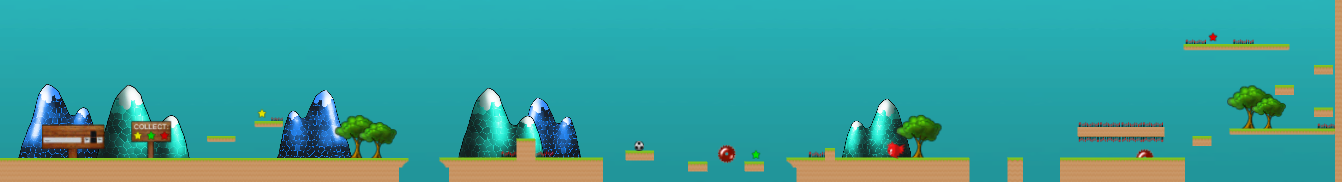
\includegraphics[width=1\textwidth]{Pics/levelStructure}
\caption{Participants played the same level four times.}
\label{fig:level}
\end{figure*}

Each time players collect three stars, the game is paused and a questionnaire is shown (see Figure \ref{fig:questionnaire}). The questionnaire consists of three sets of questions. The first asks players to try and describe the feeling of controlling the ball on the ground and in the air, with their own words. It is stressed that the chosen word(s) should be something that the player would use to describe the feeling to a friend. There were no restrictions on what types of words players could use (the input field's length is equivalent to approximately 66 characters, but it is possible to scroll forward/backward if a participant writes more than this). Each input field includes five randomly-chosen example words to give participants an idea of what could be used (see Table \ref{table:wordsExamples}). Participants were asked to describe the feeling both on the ground and in air. Even though only horizontal movement is changed in the form of the acceleration and deceleration (both apply on ground and in air), there is a possibility that players perceived the game feel differently on ground and in air. Instead of trying to describe both at the same time, players were shown two input fields.

\begin{table} \centering
\scriptsize
\caption{Participants were shown five randomly-chosen words to give them an idea of what they could write.}
\label{table:wordsExamples}
\begin{tabular}{ccccc}
\toprule
Fragile & Rigid & Firm & Solid & Thick\\
Fixed & Robust & Sore & Steadfast & Wild\\
Constant & Free & Hard & Tough & Restricted\\
Limited & Reduced & Fast & Heavy & Slow\\
Enjoyable & Stressful & Annoying & Realistic & Normal\\
Difficult & Easy & Dry & Juicy & Mechanical\\
Automatic & Organic & Exciting & Wet & Simple\\
Complicated & Direct & Inert & Unrealistic & Light\\
\bottomrule
\end{tabular}
\end{table}

After describing the game feel with the players' own words, a new set of questions was shown. Here, players were asked to rate the game feel on a 7-point Likert scale. Taking inspiration from Swink \cite{swink}, players rated the game feeling on how \textit{twitchy}, \textit{fluid}, \textit{stiff}, \textit{floaty} and \textit{responsive} they felt the controls were. Lastly, players were asked about how \textit{enjoyable}, \textit{difficult} and \textit{frustrating} it was to control the ball, as well as \textit{how much they liked} the control of the ball. In case players forgot how it felt to control the ball, they could always click on the \textit{Resume Playing} button to refresh their memories before continuing with the questionnaire.

After finishing the fourth round, participants were asked to complete an online post-questionnaire. The questions here were about game feel in general.

\begin{figure*}[htbp]
\centering
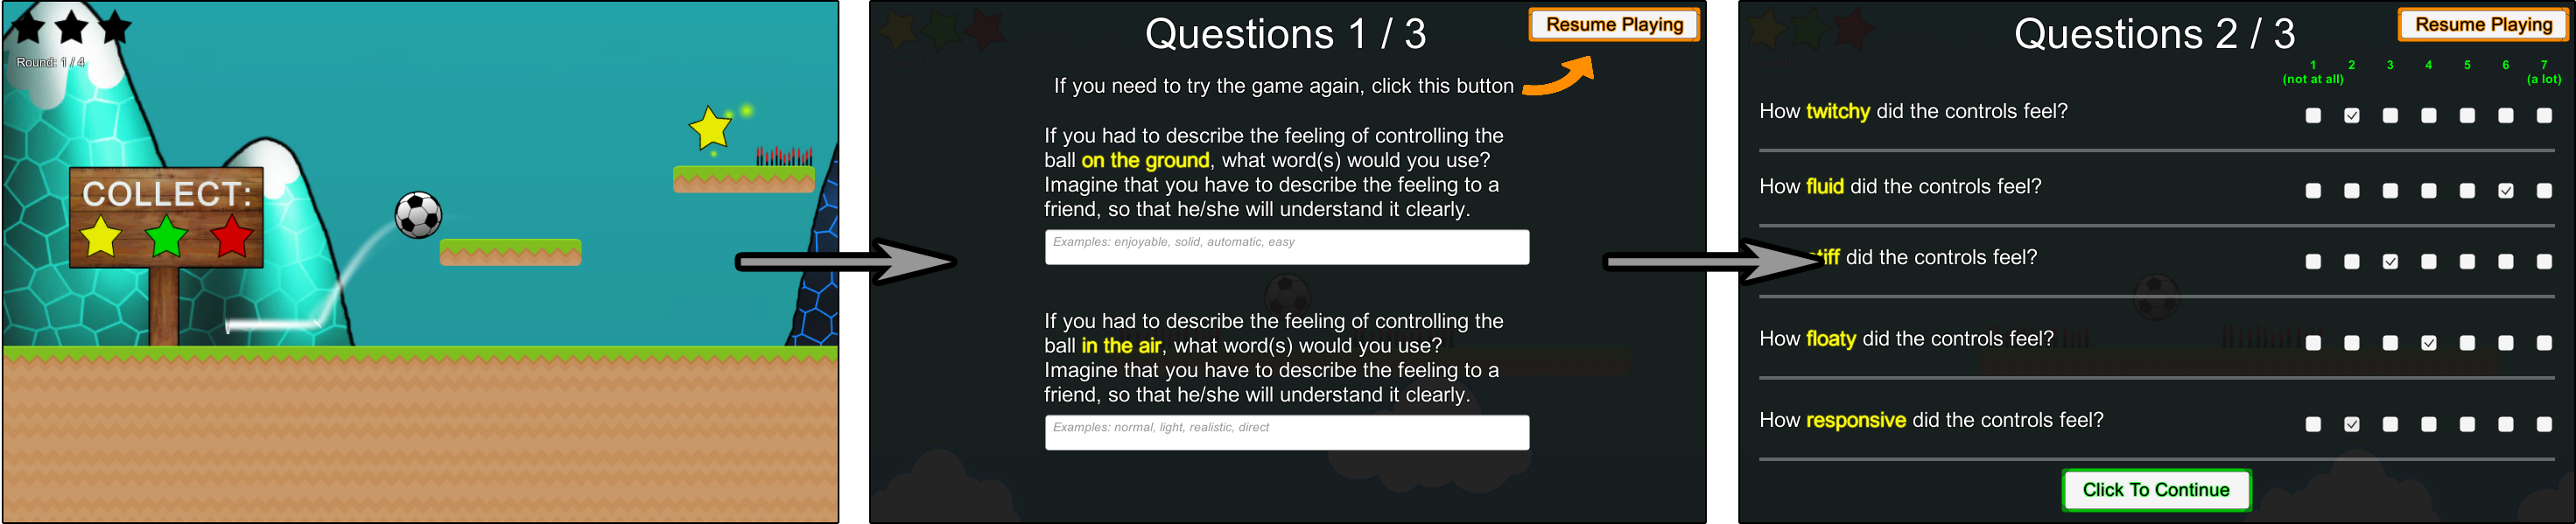
\includegraphics[width=0.95\textwidth]{Pics/game_phases}
\caption{When the player collected three stars, the game paused and showed a questionnaire.}
\label{fig:questionnaire}
\end{figure*}

\subsection{Participants}
The game was uploaded to a server and shared on social media websites and gaming forums. The primary target group was people who already play videogames; however, others were welcome to play the game as well. The participants were oblivious to the exact purpose and methods used in the experiment; they only knew that the research topic was about game feel (however, the term was never explained), but not how this was measured.

A web page\footnote{The game is available here: \\ \url{http://tunnelvisiongames.com/g/GameFeel.html}} was created where participants could choose to either play the game in their browser or download a standalone build. Whenever a player completed a round (by collecting three stars and answering the questionnaire), data was sent to an MySQL database.
%To ensure the order in the Latin square (see Section \ref{latinSection}), players were assigned a number between 1 and 4 when starting the game. This number corresponds to the sequences in Table \ref{table:latin}. This was achieved by taking modulus 4 of the total amount of participants having completed the experiment and adding 1 to it. For instance, if 26 participants had played the game before entering, the next player would be assigned the sequence number (26 \% 4) + 1 = 3.